\documentclass{llncs}
\usepackage{fullpage}
\usepackage{float}
\usepackage{tikz}
\usepackage{amsmath}
\usetikzlibrary{arrows}

\usepackage{enumitem}
\usepackage{graphicx}
\usepackage{array}
\usepackage{booktabs}
\usepackage[utf8]{inputenc}

% Redefine las subsecciones para usar letras en lugar de números
\usepackage{titlesec}
\renewcommand\thesubsection{\alph{subsection})}

\begin{document}

\title{Planificación de tareas}

\author{Miguel Ángel Dorado Maldonado}
\institute{\email{miguelangeldorado10@uma.es} \\
TCIS. Universidad de Málaga.}

\maketitle 

\vspace{1cm} 

\section{Un proyecto viene especificado por el siguiente orden de precedencia de sus actividades:}

\begin{align*}
B &\longrightarrow C \\
A, B &\longrightarrow D \\
C, D &\longrightarrow E \\
A, B &\longrightarrow F \\
F &\longrightarrow G \\
E, G &\longrightarrow H \\
H &\longrightarrow I \\
\end{align*}

\begin{enumerate}

	\item[a)] Realice un diagrama con la programación de las actividades.

		\begin{figure}[H]
		\centering
		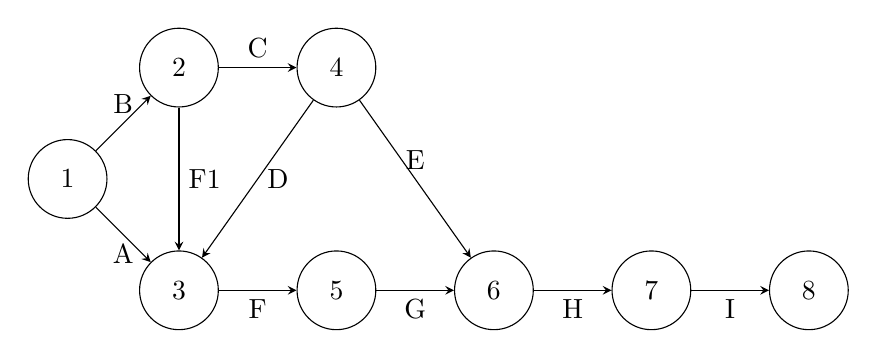
\begin{tikzpicture}[->, >=stealth, node distance=2cm, state/.style={circle, draw, minimum size=1cm}]

		\node[state] (1) {1};
		\node[state] (2) [above right of=1] {2};
		\node[state] (3) [below right of=1] {3};
		\node[state] (4) [right of=2] {4};
		\node[state] (5) [right of=3] {5};
		\node[state] (6) [right of=5] {6};
		\node[state] (7) [right of=6] {7};
		\node[state] (8) [right of=7] {8};

		\path 
		(1) edge node[above] {B} (2)
				edge node[below] {A} (3)
		(2) edge node[above] {C} (4)
				edge node[right] {F1} (3)
		(3) edge node[below] {F} (5)
		(4) edge node[right] {D} (3)
				edge node[above] {E} (6)
		(5) edge node[below] {G} (6)
		(6) edge node[below] {H} (7)
		(7) edge node[below] {I} (8);

		\end{tikzpicture}
		\caption{Diagrama de precedencia de actividades}
		\end{figure}

	\item[b)] Suponga el siguiente cuadro de duraciones para cada actividad.

		\begin{center}
		\begin{tabular}{|c|ccccccccc|}
			\hline
			Actividad & A & B & C & D & E & F & G & H & I \\
			\hline
			Duración (días) & 3 & 1 & 2 & 1 & 10 & 2 & 8 & 6 & 3 \\
			\hline
		\end{tabular}
		\end{center}
		Determine la duración del proyecto y su camino crítico.
		\\

	\item[c)] Obtenga el diagrama de Gantt.

\end{enumerate}

\section{Considere el proyecto que viene determinado por el siguiente diagrama con la programación de sus actividades.}

\begin{figure}[H]
	\begin{center}
		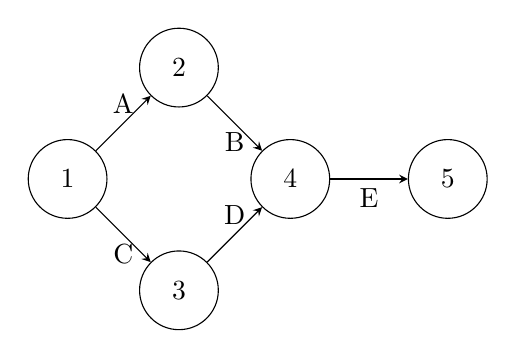
\begin{tikzpicture}[->, >=stealth, node distance=2cm, state/.style={circle, draw, minimum size=1cm}]

		\node[state] (1) {1};
		\node[state] (2) [above right of=1] {2};
		\node[state] (3) [below right of=1] {3};
		\node[state] (4) [below right of=2] {4};
		\node[state] (5) [right of=4] {5};

		\path 
		(1) edge node[above] {A} (2)
				edge node[below] {C} (3)
		(2) edge node[below] {B} (4)
		(3) edge node[above] {D} (4)
		(4) edge node[below] {E} (5);

		\end{tikzpicture}
	\end{center}
\end{figure}


\begin{enumerate}
	\item[a)] Suponga el siguiente cuadro de duraciones para cada actividad.

		\begin{center}
			\begin{tabular}{|c|ccccc|}
				\hline
				Actividad & A & B & C & D & E \\
				\hline
				Duración (días) & 3 & 4 & 2 & 6 & 3 \\
				\hline
			\end{tabular}
		\end{center}

	\item[b)] Suponga que no se conoce la duración de las actividades de forma determinista pero se estiman los siguientes tiempos optimista ($t_o$), más probable ($t_m$) y pesimista ($t_p$).

		\begin{center}
			\begin{tabular}{|c|c@{\hspace{0.3cm}}c@{\hspace{0.3cm}}c|}
					\hline
					Actividad & t_o & t_m & t_p \\
					\hline
					A & 2 & 5 & 8 \\
					B & 1 & 4 & 6 \\
					C & 2 & 2 & 3 \\
					D & 4 & 6 & 9 \\
					E & 3 & 5 & 7 \\
					\hline
			\end{tabular}
		\end{center}

\end{enumerate}

\end{document}

